\section{Supplementary Figures}
\label{app:supplementary_figures}
    \begin{figure}[ht!]
      \centering
        \includesvg[width=\textwidth]{sample_distribution_within_germany}
        \caption{Geographic distribution of sequences within Germany}
        \label{fig:geographic_sequence_distribution}
    \end{figure}
    \clearpage
    \begin{figure}[ht!]
      \centering
        \includesvg[width=.9\textwidth]{clade_distribution_over_time}
        \caption{Seasonal clade distribution}
        \label{fig:clade_distribution_over_time}
    \end{figure}
    \begin{figure}[ht!]
      \centering
        \includesvg[width=.9\textwidth]{median_amount_per_federal_state}
        \caption{Geographic distribution of mutations per sequence}
        \label{fig:median_mutations_per_federal_state}
    \end{figure}
    \clearpage
\begin{figure}[ht!]
  \centering
    \begin{subfigure}[b]{0.495\textwidth}
            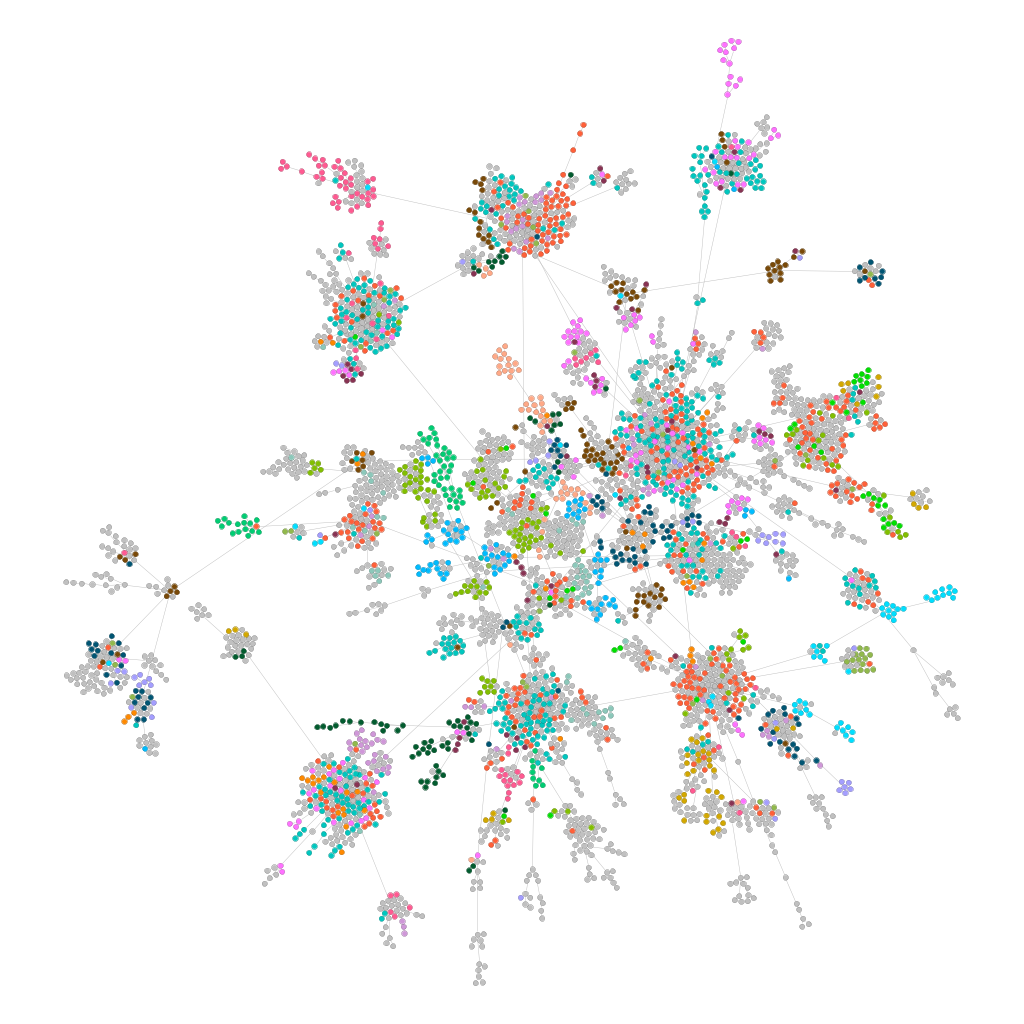
\includegraphics[width=\linewidth]{ari_test_0.1}
    \caption*{$\text{ARI}_{com}$ = 0.1}
    \end{subfigure}
    \hfill
    \begin{subfigure}[b]{0.495\textwidth}
            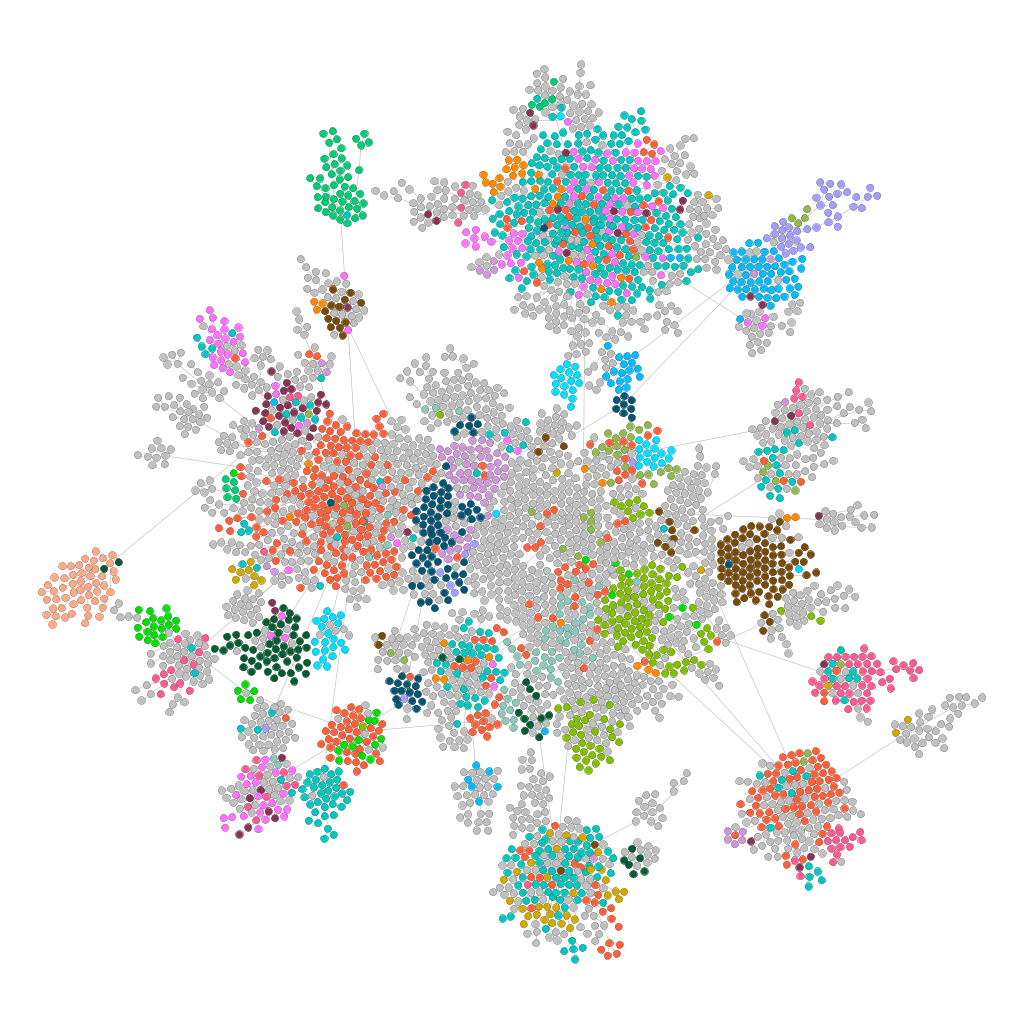
\includegraphics[width=\linewidth]{ari_test_0.3}
    \caption*{$\text{ARI}_{com}$ = 0.3}
    \end{subfigure}
  \hfill
    \begin{subfigure}[b]{0.495\textwidth}
            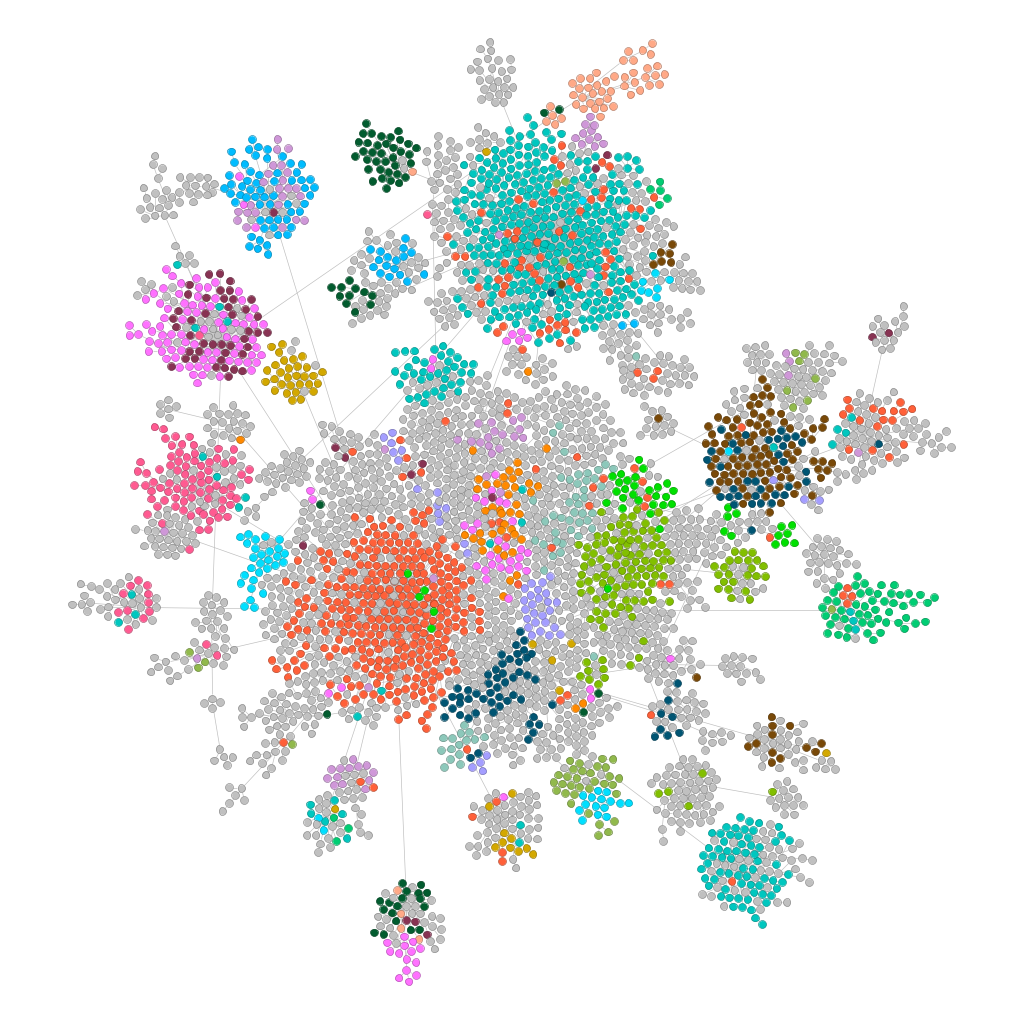
\includegraphics[width=\linewidth]{ari_test_0.5}
    \caption*{$\text{ARI}_{com}$ = 0.5}
    \end{subfigure}
  \hfill
    \begin{subfigure}[b]{0.495\textwidth}
            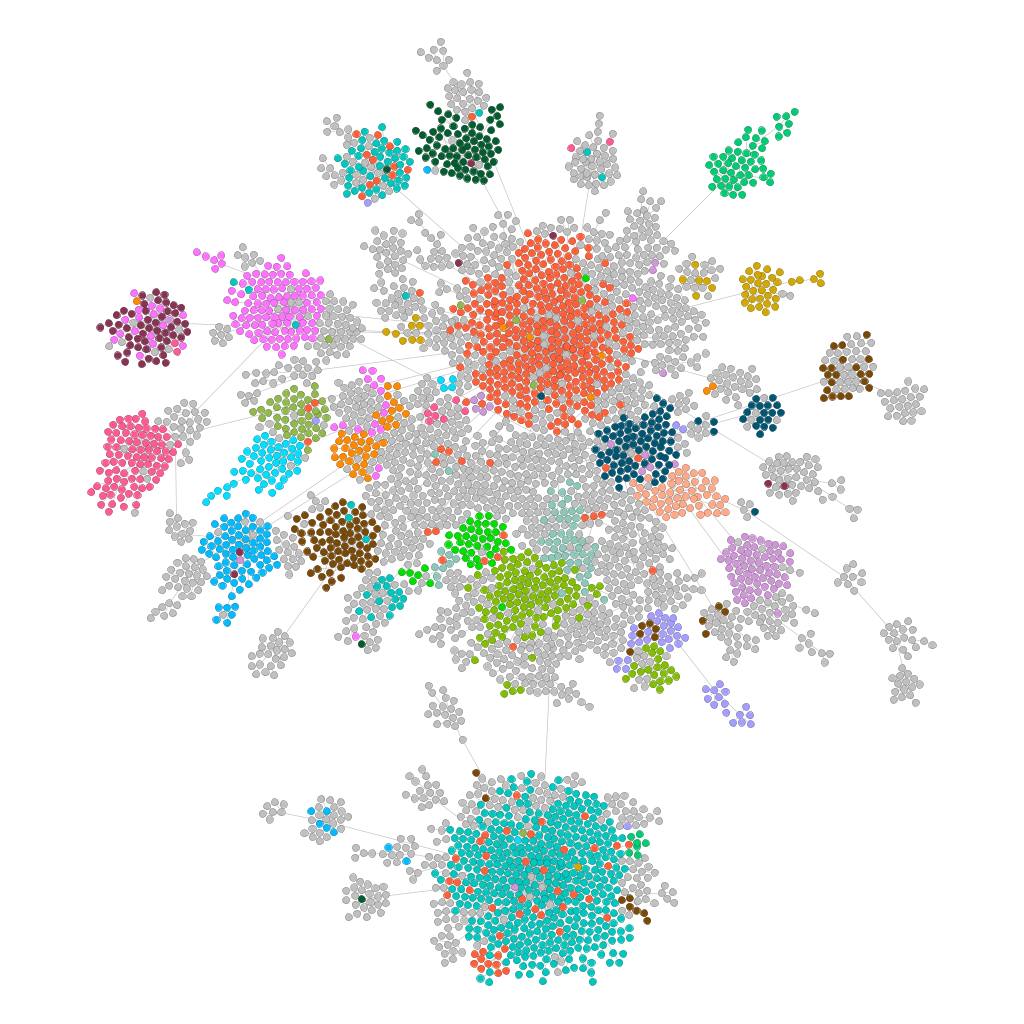
\includegraphics[width=\linewidth]{ari_test_0.7}
    \caption*{$\text{ARI}_{com}$ = 0.7}
    \end{subfigure}
    \caption{Impact of community \acrshort{ari} scores}
    \label{fig:community_ari_impact}
\end{figure}
\clearpage
  \begin{figure}[ht!]
  \centering
    \begin{subfigure}[b]{.8\textwidth}
            \includesvg[width=\linewidth]{optimized_dates_nrw_2022_10000}
    \caption*{(a) Sampling dates}
    \end{subfigure}
    \par\vspace{1em}
    \begin{subfigure}[b]{.8
    \textwidth}
            \includesvg[width=\linewidth]{optimized_cities_nrw_2022_10000}
    \caption*{(b) Cities of collection}
    \end{subfigure}
    \caption{Large-scale version of $T$\textsubscript{mod} for nrw\_2022 with 10,000 sequences}
    \label{fig:large_scale_sampling_date_optimized}
    \end{figure}
    \clearpage
  \begin{figure}[ht!]
  \centering
    \begin{subfigure}[b]{.8\textwidth}
            \includesvg[width=\linewidth]{lsh_nrw_2022_10000_dates}
    \caption*{(a) Sampling dates}
    \end{subfigure}
    \par\vspace{1em}
    \begin{subfigure}[b]{.8\textwidth}
            \includesvg[width=\linewidth]{lsh_nrw_2022_10000_cities}
    \caption*{(b) Cities of collection}
    \end{subfigure}
    \caption{Large-scale version of $T$\textsubscript{ACS} for nrw\_2022 with 10,000 sequences}
    \label{fig:large_scale_sampling_date_acs}
    \end{figure}
    \clearpage
\section{Supplementary Tables}
    \label{app:supplementary_tables}
    \begin{table}[ht!]
        \caption{Complete infection recall and community \acrshort{ari} scores for \acrshort{ccs}}
        \label{table:ccs_scores}
    \small
        \rotatebox{90}{%
            \begin{tabular}{c|c|c|c|c|c|c|c|c|c|c}
                \multirow{3}{*}{Search strategy}&\multicolumn{2}{c|}{Aggregate}& \multicolumn{8}{c}{Calculation rate}\\
                \cline{2-11}
                &\multirow{2}{*}{Size} & \multirow{2}{*}{Label} & \multicolumn{2}{c|}{0.05} & \multicolumn{2}{c|}{0.1} & \multicolumn{2}{c|}{0.15} & \multicolumn{2}{c}{0.2}\\
                \cline{4-11}
                &&&$\text{R}_{inf}$ & $\text{ARI}_{com}$ & $\text{R}_{inf}$ & $\text{ARI}_{com}$ & $\text{R}_{inf}$ & $\text{ARI}_{com}$ & $\text{R}_{inf}$ & $\text{ARI}_{com}$ \\
                \hline    
                \hline    
                Depth search&1,250& due\_202203 & 0.787 & 0.17 & 0.854 & 0.31 & 0.904 & 0.365 & 0.935 & 0.444 \\
                 \cline{3-11}
                && nrw\_202203 & 0.722 & 0.134 & 0.852 & 0.26 & 0.925 & 0.39 & 0.946 & 0.464 \\
                 \cline{3-11}
                && due\_2022 & 0.864 & 0.354 & 0.934 & 0.524 & 0.979 & 0.688 & 0.986 & 0.774 \\
                 \cline{3-11}
                && nrw\_2022 & 0.918 & 0.477 & 0.907 & 0.701 & 0.987 & 0.758 & 0.993 & 0.786 \\
                \cline{2-11}        
                & 2,500 & due\_202203 & 0.763 & 0.48 & 0.857 & 0.672 & 0.914 & 0.696 & 0.941 & 0.758 \\
                \cline{3-11}
                && nrw\_202203 & 0.764 & 0.212 & 0.867 & 0.323 & 0.915 & 0.429 & 0.947 & 0.511 \\
                \cline{3-11}
                && due\_2022 & 0.905 & 0.408 & 0.975 & 0.532 & 0.986 & 0.541 & 0.988 & 0.604 \\
                 \cline{3-11}
                && nrw\_2022 & 0.92 & 0.493 & 0.976 & 0.692 & 0.99 & 0.787 & 0.995 & 0.872 \\
                \cline{2-11}        
                &5,000 & due\_202203 & 0.767 & 0.275 & 0.826 & 0.263 & 0.869 & 0.333 & 0.909 & 0.336 \\
                 \cline{3-11}
                && nrw\_202203 & 0.803 & 0.268 & 0.91 & 0.406 & 0.945 & 0.544 & 0.967 & 0.624 \\
                 \cline{3-11}
                && due\_2022 & 0.914 & 0.378 & 0.971 & 0.537 & 0.985 & 0.619 & 0.99 & 0.675 \\
                 \cline{3-11}
                && nrw\_2022 & 0.942 & 0.423 & 0.979 & 0.601 & 0.993 & 0.77 & 0.995 & 0.853 \\
                \hline
                \hline    
                Breadth search&1,250 & due\_202203 & 0.364 & 0.175 & 0.55 & 0.217 & 0.666 & 0.266 & 0.747 & 0.257  \\
                 \cline{3-11}
                && nrw\_202203 & 0.406 & 0.115 & 0.594 & 0.212 & 0.714 & 0.209 & 0.785 & 0.277 \\
                 \cline{3-11}
                && due\_2022 & 0.659 & 0.318 & 0.801 & 0.43 & 0.873 & 0.43 & 0.911 & 0.528 \\
                 \cline{3-11}
                && nrw\_2022 & 0.768 & 0.472 & 0.894 & 0.549 & 0.929 & 0.617 & 0.937 & 0.769 \\
                \cline{2-11}        
                &2,500 & due\_202203 & 0.407 & 0.23 & 0.597 & 0.284 & 0.709 & 0.316 & 0.786 & 0.375 \\
                \cline{3-11}
                && nrw\_202203 & 0.422 & 0.139 & 0.606 & 0.226 & 0.713 & 0.283 & 0.776 & 0.379 \\
                \cline{3-11}
                && due\_2022 & 0.715 & 0.319 & 0.849 & 0.332 & 0.907 & 0.461 & 0.933 & 0.547 \\
                 \cline{3-11}
                && nrw\_2022 & 0.772 & 0.44 & 0.882 & 0.558 & 0.932 & 0.627 & 0.959 & 0.688  \\
                \cline{2-11}        
                &5,000 & due\_202203 & 0.431 & 0.177 & 0.591 & 0.228 & 0.704 & 0.263 & 0.786 & 0.294 \\
                 \cline{3-11}
                && nrw\_202203 & 0.469 & 0.131 & 0.657 & 0.188 & 0.756 & 0.265 & 0.822 & 0.396 \\
                 \cline{3-11}
                && due\_2022 & 0.706 & 0.308 & 0.843 & 0.389 & 0.907 & 0.441 & 0.933 & 0.472 \\
                 \cline{3-11}
                && nrw\_2022 & 0.809 & 0.389 & 0.915 & 0.492 & 0.956 & 0.591 & 0.972 & 0.654 \\
            \end{tabular}  
            }    
        \end{table}
        \clearpage
\setcounter{table}{0}
\section{Code base}
The code base to this work is available in a public GitHub repository at \url{https://github.com/benjoka/thesis_bk}. Table \ref{table:code_base_structure} describes the directory structure of the code base.

\renewcommand{\arraystretch}{1.5}
\begin{table}[H]
\centering
\caption{Directory structure of the code base}
\label{table:code_base_structure}
\begin{tabular}{>{\centering\arraybackslash}p{0.2\textwidth}|>{\centering\arraybackslash}p{0.7\textwidth}}
Directory & Description \\
\hline\hline
results & Results of the thesis. Scores of \acrshort{acs} might differ from the concrete scores listed in the thesis, as the procedure does not produce unambiguous results. The order of directories reflects the order results are presented in the thesis. \\
\hline
gendisc & Golang package that implements the GENTRAIN algorithm to calculate genetic distances. When executed with \texttt{--fast} the adjustments proposed in this work are used. \\
\hline
gentrain & Python module with the implementations of the approaches proposed in the thesis and several helper functions for evaluation purposes. \\
\hline
latex & LaTeX files of the thesis. \\
\end{tabular}
\end{table}
\clearpage
\setcounter{table}{0}
\section{Software and Hardware Used}
 \begin{table}[ht!]
    \caption{Software used}
    \label{table:software}
        \begin{threeparttable}
            \begin{tabular}{Sc|Sc|Sc}
                Software & Version & Purpose \\
                \hline\hline
                GoLand & 2024.3.4 & Golang programming \\
                \hline
                PyCharm & 2024.2.5 & Python Programming, Jupyter Notebooks \\
                \hline
                scikit-learn & 1.6.1 & Data analysis \\
                \hline
                pandas & 2.2.3 & Data analysis and manipulation \\
                \hline
                NumPy & 2.0.0 & Data analysis and manipulation \\
                \hline
                jupyter & 1.1.1 & Results preparation and presentation \\
                \hline
                HNSWlib & 0.8.0 & \acrshort{acs} benchmarking \\
                \hline
                Biopython & 1.85 & Fasta file processing \\
                \hline
                NetworkX & 3.4.2 & Graph creation and manipulation \\
                \hline
                Plotly & 6.2.0 & Plot creation \\
                \hline
                Gephi & 0.10.1 & Graph visualization and configuration \\
                \hline
                Adobe Illustrator & 29.5 & SVG processing \\
                \hline
                Canva & - & Aggregate figure creation \\
                \hline
                Deepl Write\textsuperscript{a} & - & AI-driven grammar and spelling correction \\
                \hline
                Writefull\textsuperscript{a} & - & AI-driven grammar and spelling correction \\
                \hline
                Google Scholar & - & Literature research \\
                \hline
                Consensus\textsuperscript{a} & - & AI-driven literature research \\
            \end{tabular}
            \begin{tablenotes}[flushleft]
                \small
                \item[a] AI tools were used with careful supervision and all scientific contributions are solely my own.
            \end{tablenotes}
        \end{threeparttable}
\end{table}
 \begin{table}[ht!]
    \caption{Hardware used}
    \label{table:hardware}
    \resizebox{\textwidth}{!}{%
        \begin{tabular}{Sc|Sc|Sc|Sc}
        Model & Processor (CPU) & Memory (RAM) & Operating System \\
        \hline\hline
        MacBook Air (2020) & Apple M1, 8-core CPU & 16 GB & macOS Sonoma 14.2.1\\
        \end{tabular}
    }
\end{table}
